
% !TEX root = main.tex

\chapter{The basics of StabFem }


In this chapter we explain the basic functionalities of StabFem. We recommend that you study the basic example \texttt{EXAMPLE\_Lshape.m}.

This directory contains three freefem programs and a demo matlab script doing solving tghe following problem :


\section{Simple problem : solution of heat equation in a L-shaped domain}

1. Solve the steady heat conduction equations on a L-shaped domain with constant volumic source term $P$ and homogeneous Dirichlet boiundary conditions :

$$ \nabla^2 T = P  \mbox {  for } {\bf x} \in \Omega ; \quad T = 0   \mbox {  for } {\bf x} \in \Gamma$$

2.  Solve the unsteady heat conduction equations on a L-shaped domain with zero source term $P$ and time-periodic Dirichlet boundary conditions :

$$ 
 \partial T_1/\partial t= \nabla^2 T_1  \mbox {  for } {\bf x} \in \Omega ; \quad T_1 = T_w e^{i \omega t}   \mbox {  for } {\bf x} \in \Gamma
$$



\section{Matlab script and results}

The programs are sufficiently short to be fully given in these pages. See figures \ref{SCRIPT_Lshape.m}, etc...

The reader already familiar with FreeFm++ should not have any provblem in undersanding the programs. If not, we recommand that you study the FreeFem++ Manual (chapter "Learning by examples").

The results are given 


\begin{figure*}[t]
\small
\lstinputlisting{../EXAMPLE_Lshape/SCRIPT_Lshape.m}
 \normalsize
\caption{
Matlab program {\texttt SCRIPT\_Lshape.m})}
\label{SCRIPT_Lshape.m}
\end{figure*}


\begin{figure*}[t]
\small
\lstinputlisting{../EXAMPLE_Lshape/Lshape_Mesh.edp}
 \normalsize
\caption{
FreeFem++ program {\texttt Lshape\_Mesh.edp})}
\label{Lshape_Mesh.edp}
\end{figure*}

\begin{figure*}[t]
\small
\lstinputlisting{../EXAMPLE_Lshape/Lshape_Steady.edp}
\normalsize
\caption{
FreeFem++ program {\texttt Lshape\_Steady.edf})}
\label{Lshape_Mesh.edp}
\end{figure*}

\begin{figure*}[t]
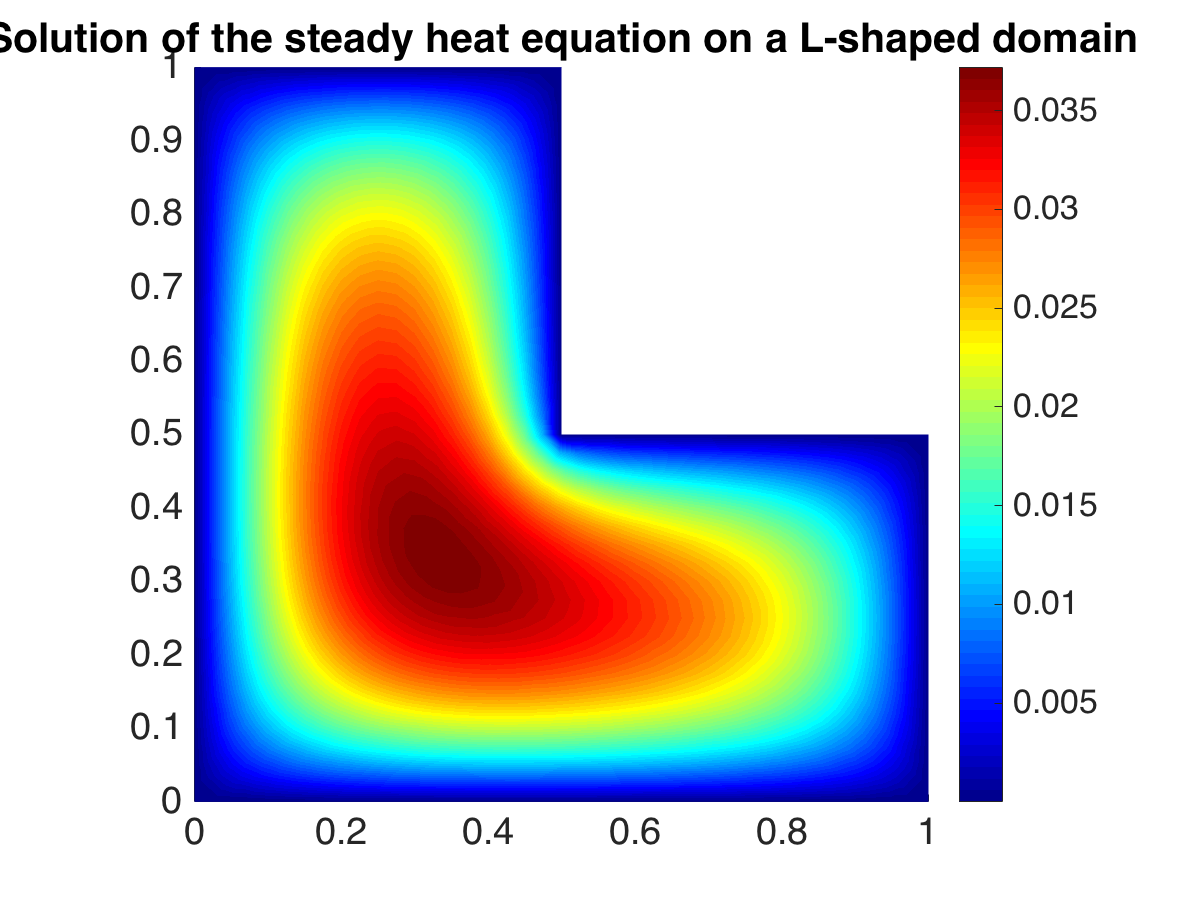
\includegraphics[width = .45 \linewidth]{../EXAMPLE_Lshape/FIGURES/Lshape_T0.png}
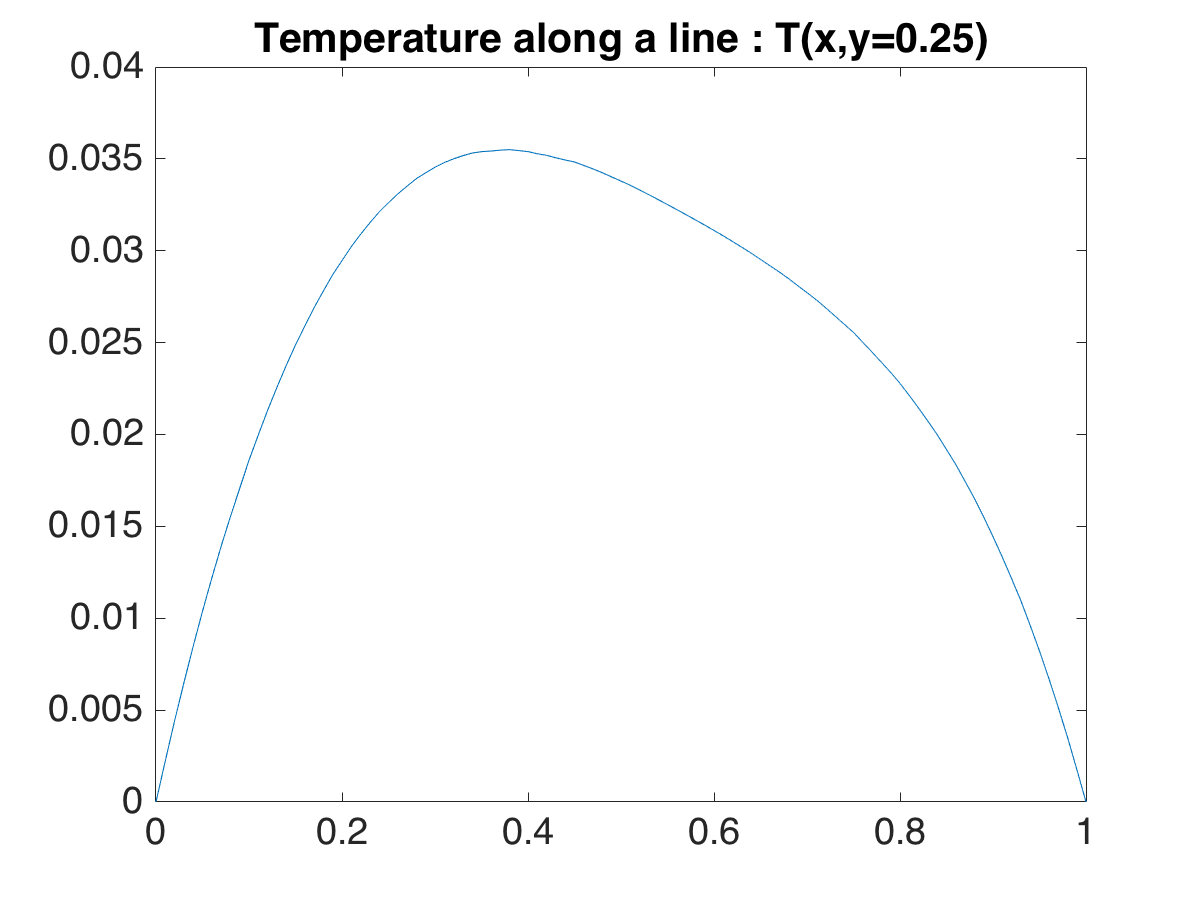
\includegraphics[width = .45 \linewidth]{../EXAMPLE_Lshape/FIGURES/Lshape_T0_Cut.png}
\caption{Solution for the steady hrat equation in a L-shape domain : $(a)$ Temperature field $T(x,y)$. 
$(b)$ Temperature $T(x,0.25)$ along a horizontal line. }
\label{Lshape_Mesh.edp}
\end{figure*}


\section{How does it work ?}


\subsection{Explanation of the \texttt{.ff2m} exchange format}.




